\theoremstyle{definition}
\newtheorem{definition}{Definition}
\newtheorem{example}[definition]{Example}
\newtheorem{note}[definition]{Note}

\theoremstyle{plain}
\newtheorem{theorem}[definition]{Theorem}
\newtheorem{lemma}[definition]{Lemma}
\newtheorem{proposition}[definition]{Proposition}
\newtheorem{corollary}[definition]{Corollary}

\newcommand{\RR}{\ensuremath{\mathbb{R}}}
\newcommand{\ZZ}{\ensuremath{\mathbb{Z}}}
\newcommand{\lapu}{\ensuremath{\mathcal{L}^{\text{up}}}}
\newcommand{\lapd}{\ensuremath{\mathcal{L}^{\text{down}}}}
\newcommand{\lap}{\ensuremath{\mathcal{L}}}
\newcommand{\iso}{\ensuremath{\cong}}

\newcommand{\ie}{}
\def\ie/{i.e.}
\newcommand{\eg}{}
\def\eg/{e.g.}
\newcommand{\etc}{}
\def\etc/{etc.}

\newcommand{\fix}[2]{{\color{red}#1}\fxfatal{#2}}
\newcommand{\suchthat}{\ensuremath{\, \mid \,}}

\newcommand{\ip}[2]{\ensuremath{\left\langle #1 , #2 \right\rangle}}

\newcommand{\placeholderfigure}{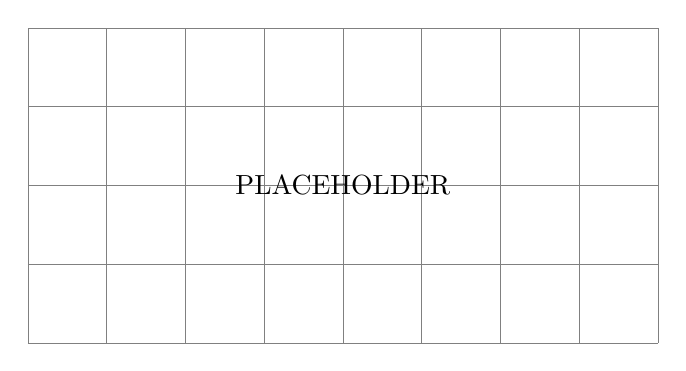
\begin{tikzpicture}
      \draw[help lines] (0, 0) grid (8, 4);
      \node () at (4,2) {PLACEHOLDER};
  \end{tikzpicture}
}
